\documentclass{article}
\usepackage[12pt]{extsizes}
\usepackage[T2A]{fontenc}
\usepackage[utf8]{inputenc}
\usepackage[english, russian]{babel}
\usepackage[left=3cm,right=1.5cm,top=2cm,bottom=2cm]{geometry}
\usepackage{hyperref}
\usepackage{amssymb,amsmath,amsthm}
\usepackage{cleveref}
\usepackage{caption}
\usepackage{mathtools}


\usepackage{graphicx}

%\полуторный интервал
\usepackage{setspace}
\onehalfspacing

%простое дерево
\usepackage{dirtree}

%формулы
\usepackage{mathtools}
% \everymath{\displaystyle}

%красные строки (не рекомендуется)
% \parindent = 1,25cm
% \usepackage{indentfirst}



%some commands for better experience
\theoremstyle{definition}
\newtheorem{define}{Определение}
\newcommand*{\defi}[1]{\begin{define} #1 \end{define}}

\theoremstyle{plain}
\newtheorem{theorem}{Теорема}
\newcommand*{\thrm}[1]{\begin{theorem} #1 \end{theorem}}

\theoremstyle{plain}
\newtheorem{lemma}{Лемма}
\newcommand*{\lemm}[1]{\begin{lemma} #1 \end{lemma}}

\newcommand*{\prf}[1]{\begin{proof} #1 \end{proof}}

\theoremstyle{plain}
\newtheorem{example}{Пример}
\newcommand*{\exmp}[1]{\begin{example} #1 \end{example}}

\newcommand*{\R}{\mathbb{R}}
\newcommand*{\und}[2]{\underset{#1}{#2}}


\begin{document}
\tableofcontents
\newpage

\section{Описание системы}
\subsection{Слой}
Каждый слой представляет из себя кластер Kubernetes из нескольких машин. Одна из машин выступает как контролер (control plane) и другие как исполнители (worker). После создания кластера посредством kubeadm, требуется установить приложения, необходимые для работы системы Dcache.
И после этого разворачивается система Dcache состоящая из двух составных частей: двери, обеспечивающей доступ к системе, и пула для хранения информации.\\
Также для обеспечения коммуникации внутри кластера Kubernetes и возможности доступа снаружи (для сервиса перемещения), требуется создание сервисов перенаправления портов.\\
После того как система запущена, требуется выбрать протокол коммуникации, который реализован в сервисе перемещения, в данном примере используется протокол webdav. 
\subsection{Сервис перемещения данных}
Для того чтобы организовать перемещение данных между двумя системами Dcache на двух слоях, описанных выше, требуется средство способное использовать либо API системы хранения либо операции: записи, чтения и удаления. Для общности примера выбран второй вариант, так как при наличии подходящих протоколов, есть возможность использовать любую другую систему хранения.\\
Для реализации использовался язык программирования python. Так как вся система ориентируется на облачные технологии выбран стек, позволяющий реализовать микросервисную архитектуру. В данном примере Backend и методы записи с помощью протоколов реализованы в одном приложении, но в практической реализации следует их разделить.\\
Серверная часть предоставляется библиотекой flask, а реализация коммуникации через протокол webdav сделана через библиотеку requests.\\
Для данного прототипа реализован минимальный набор API:
\begin{itemize}
    \item upload [POST] - загружает файл в хранилище с номером 1, а также записывает метаданные в свое локальное хранилище.
    \item move [POST] - перемещает файл с указанным в запросе id, в хранилище с указанным номером. 
    \item files [GET] - возвращает список, всех файлов в формате json с описаниями места хранения и пути для получения файла.
\end{itemize}
Для загрузки файла пользователь напрямую обращается к нужному хранилищу посредством протокола webdav. \\
Также важно отметить, что сервису необходимо знать о портах доступных для записи поддерживаемым протоколом, которые организуются в кластере посредством сервисов перенаправления портов, описанных выше. 

\section{Реализация}
\subsection{Кластер Kubernetes}
Наиболее важным источником информации в данном вопросе является: \url{https://kubernetes.io/docs/setup/production-environment/tools/kubeadm/create-cluster-kubeadm/} - официальная документация kubernetes. Также кластер можно разворачивать 
любыми средствами. В данном примере используется \textbf{kubeadm}.  Для того чтобы развернуть систему через kubeadm нужно:
\begin{itemize}
   \item \textbf{Ознакомится с документацией инструмента развертывания}
   \item Подготовить средство запуска контейнеров containerd или docker \\
   Для установки containerd следует пользоваться руководством: \url{https://github.com/containerd/containerd/blob/main/docs/getting-started.md}\\
   Также следует сделать настройку cgroup описанную \url{https://kubernetes.io/docs/setup/production-environment/container-runtimes/#containerd}.
   \item Отключить swap и установить инструменты kubectl и kubelet\\
   Инструкции здесь \url{https://kubernetes.io/docs/setup/production-environment/tools/kubeadm/install-kubeadm/}
   \item Выбрать сетевой аддон\\
   Список адонов тут \url{https://kubernetes.io/docs/concepts/cluster-administration/addons/#networking-and-network-policy}. В данной реализации используется 
   flannel. Для его установки следует следовать гайду \url{https://github.com/flannel-io/flannel#deploying-flannel-manually}. Важно отметить что нужно указать podCidr при инициализации 
   кластера (Подробно по ссылке).
   \item Сеть\\
   Также может потребоваться отключение фаерволла. В almalinux: sudo systemctl stop firewalld. Либо открыть все необходимые порты?
   \item Создать кластер через команды kubeadm init и kubeadm join.
\end{itemize}
После создания кластера команды kubectl get nodes и kubectl get pods должны работать и не выдавать ошибки. Иначе следует пересоздать кластер и следовать инструкции (более тщательно?).
Пример работы:
\begin{figure}[h]
   \centering
   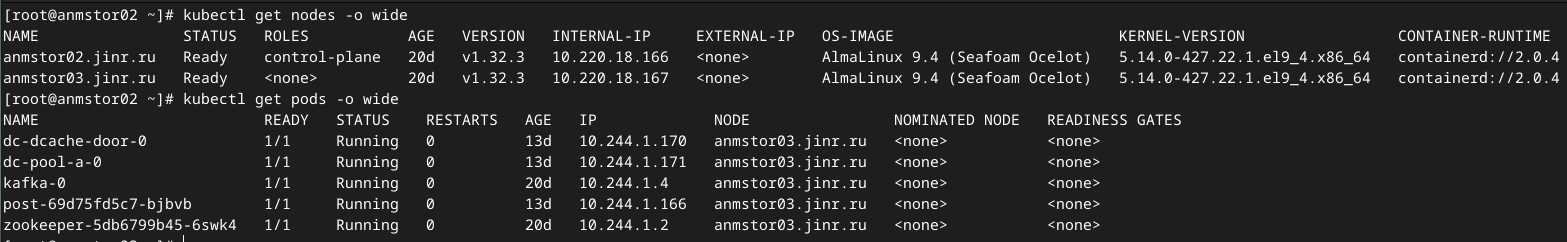
\includegraphics[width=0.8\textwidth]{images/examp.png}
   \caption{Тест кластера}
\end{figure}\\
Также следует понимать для организации перемещения \textbf{потребуется несколько кластеров dcache} В данном примере используются два отдельных кластера kubernetes на разных машинах, но данное решение можно реализовать и в разных пространствах имен одного кластера (потребуется перенаправить сервисами порты).

\subsection{Запуск Dcache на кластере}
Репозиторий с кодом \url{https://github.com/sxvxmx/dcachelayer}.
\subsubsection{Вспомогательные сервисы}
После того как \textbf{кластер развернут} необходимо подготовить приложения для запуска dcache а именно:
\begin{itemize}
   \item Postgresql с пользователем chimera для хранения метаданных
   \item Zookeeper для коммуникации
   \item Kafka для обработки сообщений
   \item Volume Claim для выдачи дискового пространства под pool. В данном примере используется локальное хранение.
   \item Сервисы доступа к frontend dcache и протоколам (webdav). 
\end{itemize}
Для развертывания следует использовать команду {\fontfamily{cmtt}\selectfont kubectl apply -f [file path]}.
\begin{enumerate}
   \item Для развертывания Postgresql требуется подготовленный контейнер, который уже загружен в docker hub. Или собрать свой (dockerfile в dapp/party/postgres).\\
   После этого требуется развернуть сервис и саму базу данных dapp/party/postgres/post.yaml. Сервис имеет название chimera-postgresql, которое определено в dcache чарте.
   \item Zookeeper и его сервис разворачиваются посредством dapp/party/zoo.yaml. Сервис также имеет название определенное в системе dcache. 
   \item Для Kafka используется файл dapp/party/kafka.yaml. Аналогично Zookeeper.
   \item Для локального хранения файлов:\\
   Установить и развернуть на кластере необходимые поды: \\
   \begin{verbatim} kubectl apply -f https://raw.githubusercontent.com/rancher/
      local-path-provisioner/master/deploy/local-path-storage.yaml \end{verbatim}
   После этого сделаем локальный путь по умолчанию: \begin{verbatim} kubectl patch storageclass local-path -p '{"metadata": {"annotations":
       {"storageclass.kubernetes.io/is-default-class":"true"}}}' \end{verbatim}
   {\fontfamily{cmtt}\selectfont kubectl get pod -n local-path-storage}\\
   Для проверки запустились ли нужные поды.\\
   {\fontfamily{cmtt}\selectfont kubectl get storageclass}\\
   Проверка того что используется локальный путь.\\
   После этого шага при установке чарта dcache автоматически занимается пространство, а также показано что установлен локальный путь по умолчанию:
   \begin{figure}[h]
      \centering
      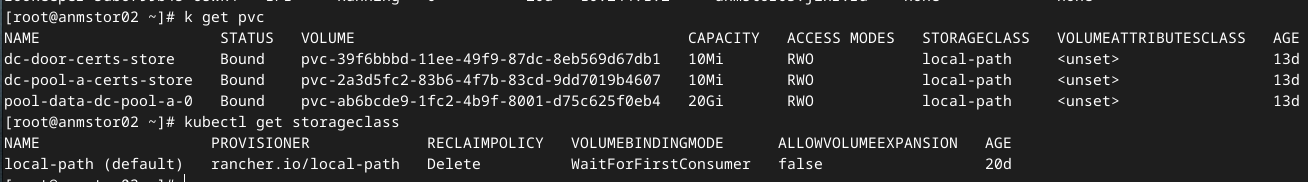
\includegraphics[width=0.8\textwidth]{images/pvc.png}
      \caption{Тест локального выделения пространства}
   \end{figure}\\
   Важно понимать что для полного удаления файлов требуется также перезапуск приложения с базой метаданных, а не только удаление локальных хранилищ.
   \item Также для доступа к dcache из внешних источников (для сервиса перемещения) требуется создать сервис, перенаправляющий порт:
   для этого применяется файл dapp/party/ webdav.yaml и dapp/party/front.yaml по аналогии можно подключить необходимый сервис из dcache вроде admin панели.
\end{enumerate}
\subsubsection{Чарт Dcache}
Чарт dcache расположен dapp/dcache-helm и является модификацией \url{https://github.com/dCache/dcache-helm}. Данный чарт создает pool-a для записи и один сервис и приложение door. 
Для установки чарта потребуется helm. Команда для установки здесь \url{https://helm.sh/docs/intro/install/}. После того как все сервисы запущены (из прошлой секции) применяется команда:
\begin{verbatim}
   helm install [name] dapp/dcache-helm/
\end{verbatim}
После чего начинается развертывание необходимых сервисов и приложений. При первом запуске также требуется загрузить контейнеры, что требует времени. На рисунке 1 показан пример запущенной системы готовой к работе.\\
Конфигурация dcache находится в dapp/dcache-helm/templates/configmap.yaml. А также dapp/dcache-helm/values.yaml -- файл позволяющий менять конфигурацию самого чарта.

\subsection{Сервис перемещения}
Сервис перемещения -- микросервис написанный на python и flask (dapp/observ). Наиболее простым способом запуска является локальный запуск python приложения через main ({\fontfamily{cmtt}\selectfont python main.py}) после установки зависимостей из requirements.txt.
Также в директории находится Dockerfile, позволяющий собрать сервис в контейнере.
\subsubsection{Использование}
Для того чтобы добавить уровни хранения в сервис требуется изменить конфигурацию в файле dapp/observ/control.py. А именно блок WEBDAV\_URLS. Для добавления новых уровней достаточно указать новое хранилище а именно его название и путь на pool в который следует записывать файлы.
\begin{figure}[h]
   \centering
   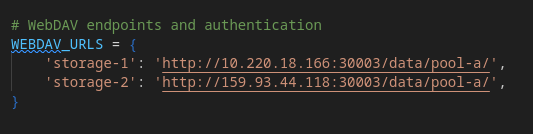
\includegraphics[width=0.8\textwidth]{images/serv.png}
   \caption{Поле ответственное за добавление хранилищ}
\end{figure}
\subsubsection{API}
Для взаимодействия сервис имеет набор из 3х эндпоинтов:
\begin{itemize}
   \item /upload - загрузка файла через post
   \item /move - перемещение файла с указанием id файла и нового хранилища
   \item /files - список всех файлов на хранилищах
\end{itemize}
Пример использования показан на рисунках:
\begin{figure}[!h]
   \centering
   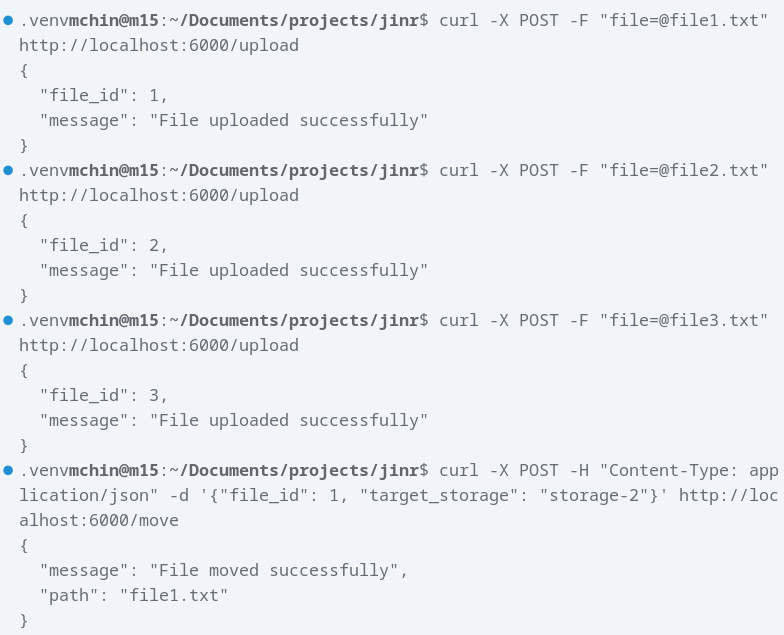
\includegraphics[width=0.6\textwidth]{images/serv1.png}
   \caption{Запись и перемещение}
\end{figure}
\begin{figure}[!h]
   \centering
   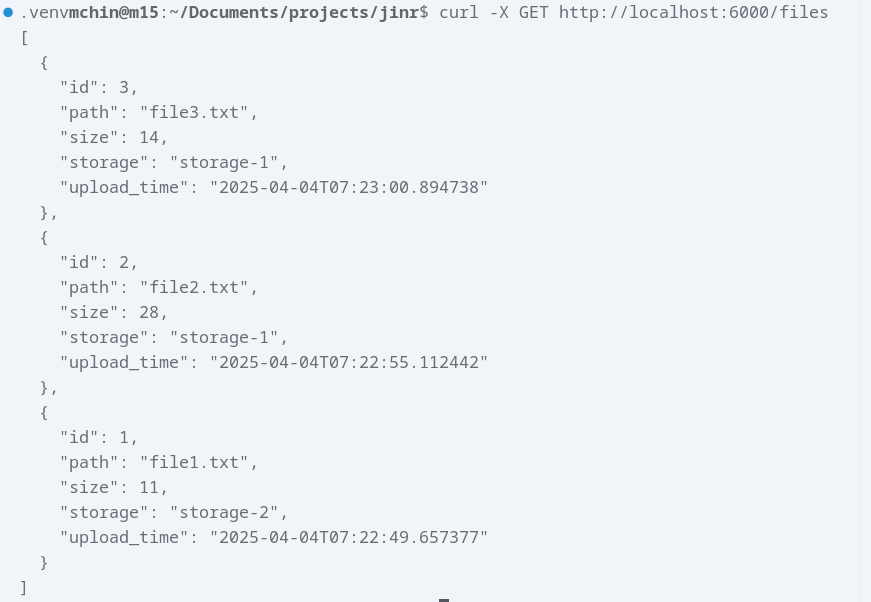
\includegraphics[width=0.6\textwidth]{images/serv2.png}
   \caption{Список файлов}
\end{figure}\\
В данном примере рассматривается система из двух слоев. Но предложенное решение никак не ограничено своей топологией. Пока каждая пара уровней связана сервисом, можно создавать любую структуру.
\newpage
\section{Dcache + docker compose}
Также в процессе разработки системы были собраны контейнеры для разных частей dcacahe. Данное решение подходит для \textbf{быстрого локального развертывания} с логическим распределением.\\
Директория compose/ является набором блоков для построения системы в среде docker compose. Файл compose/compose.yaml позволяет запустить dcache в виде трех узлов общающихся через Zookeeper в отдельном контейнере.\\
Каждая отдельная поддиректория вроде compose/dcache-core содержит dockerfile для сбора контейнера для описанного узла. Также в compose/dcache-core/config/ содержатся основные файлы конфигурации dcache для узла.
Для быстрого запуска требуется установить docker \url{https://docs.docker.com/engine/install/}. После чего выполнить в папке с compose.yaml:
\begin{verbatim}
   docker compose up --build
\end{verbatim}
Данная архитектура в точности повторяет систему описную в книге: \url{https://www.dcache.org/manuals/Book-10.0/install.shtml} к моменту распределенной системы на нескольких узлах. Следовательно можно пользоваться командами из
книги чтобы записать файл через webdav:\\
<<The WebDAV door is listening on port 2880 (the default). We can upload a file into dCache using that protocol, with the curl client.
\begin{verbatim}
curl -u tester:TooManySecrets -L -T /bin/bash 
http://localhost:2880/home/tester/test-file-1
\end{verbatim}
The file may also be downloaded:
\begin{verbatim}
curl -u tester:TooManySecrets -L -o /tmp/test-file-1 
http://localhost:2880/home/tester/test-file-1>>
\end{verbatim}
\end{document}